\section{Założenia techniczne}
\label{sec:zalozenia_techniczne}

Ze względu na charakter aplikacji, jakim jest edukacyjna gra komputerowa,
opierająca się w dużym stopniu na renderowaniu grafiki,
do wykonania projektu wybrano silnik Unity w wersji 6000.0.25f1.
Z wielu zalet silnika Unity, kluczowe dla niniejszego projektu są:

\begin{citemize}
    \item Wsparcie dla wielu platform --
    Unity pozwala na tworzenie aplikacji na wiele platform jednocześnie, w tym przede wszystkim na systemy Windows, Linux oraz macOS.
    \item Prostota tworzenia aplikacji graficznych --
    Unity oferuje wiele narzędzi, które ułatwiają tworzenie interaktywnych aplikacji graficznych,
    dzięki czemu można skupić się na tworzeniu mechanik gry.
    \item Szerokie wsparcie --
    Unity posiada rozbudowaną dokumentację~\cite{unity_docs}, aktywne forum~\cite{unity_forum} oraz wiele darmowych zasobów,.
\end{citemize}

Unity korzysta z języka C\#, opartego o paradygmat programowania obiektowego (ang. OOP — Object-Oriented Programming),
polegający na tworzeniu obiektów na podstawie abstrakcji klas, a także innych obiektów~\cite{nygaard1986basic}.
Pozwala to na tworzenie wielu obiektów o podobnych cechach, co ułatwia pisanie kodu oraz jego późniejsze utrzymanie.\\

\subsection{Architektura programu}
\label{subsec:architektura_programu}

Aby zapewnić modularność oraz separację elementów aplikacji,
wykorzystano odpowiednio zaadaptowana architekturę MVVM (Model-View-ViewModel).
Bazowo polega ona na podziale komponentów aplikacji na trzy główne części: model, widok oraz widok-model.
Funkcje każdego z nich opisano w tab.~\ref{tab:mvvm}.

\begin{table}[h]
    \centering
    \caption[Opis funkcji poszczególnych elementów architektury MVVM.]
    {Opis funkcji poszczególnych elementów architektury MVVM, źródło:~\cite{mvvm}.}
    \label{tab:mvvm}
    \begin{tabular}{|c|p{0.6\textwidth}|}
        \hline
        Element & Opis \\
        \hline
        \hline
        Widok & Odpowiada za prezentację danych oraz interakcję z użytkownikiem. \\
        \hline
        Widok-model & Odpowiada za przekazywanie danych pomiędzy modelem a widokiem. \\
        \hline
        Model & Odpowiada za przechowywanie danych oraz logikę danego komponentu programu. \\
        \hline
    \end{tabular}
\end{table}

Tak jak pierwotnie w architekturze MVVM, po adaptacji,
widok odpowiada za prezentację danych oraz interakcję z użytkownikiem.
Widok-model odpowiada za przekazywanie danych pomiędzy nie tylko między modelem a widokiem,
ale również między innymi częściami aplikacji jako menedżer danego systemu aplikacji.
Sam model natomiast składa się z wielu komponentów, które przechowują dane oraz logikę danego komponentu aplikacji.
Zarys architektury programu przedsawiono na rys.~\ref{fig:architektura}.

\begin{figure}[h]
    \centering
    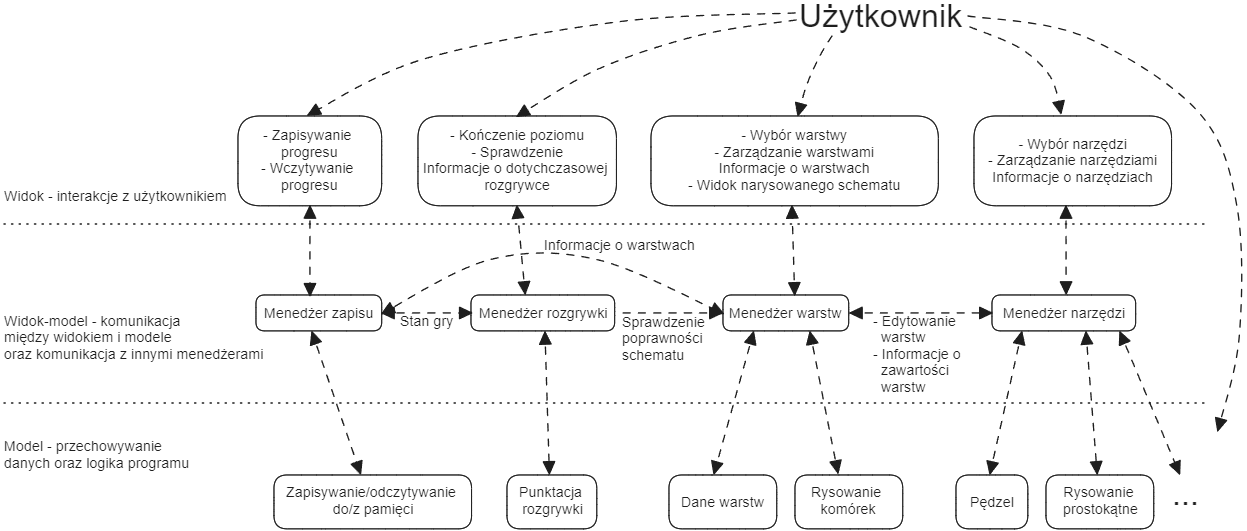
\includegraphics[width=.9\textwidth]{chapters/chapter3/rys/arch}
    \caption[Architektura programu.]{Architektura programu, źródło: opracowanie własne.}
    \label{fig:architektura}
\end{figure}